\documentclass[sigconf,review,anonymous]{acmart}

\usepackage{booktabs}
\usepackage{tabularx}
\usepackage{enumitem}
\usepackage{amsmath}
\usepackage{microtype}
\usepackage{xspace}
\usepackage{tikz}
\usetikzlibrary{arrows.meta,positioning,fit}

\settopmatter{printacmref=false,printccs=false,printfolios=true}
\setcopyright{none}
\acmYear{2027}
\acmConference[CODASPY '27]{17th ACM Conference on Data and Application Security and Privacy}{June 14--17, 2027}{Fort Collins, Colorado, USA}
\renewcommand\footnotetextcopyrightpermission[1]{}
\pagestyle{plain}
\setlength{\headheight}{16pt}
\setlength{\emergencystretch}{1.5em}

\newcommand{\U}{\textsf{U}}
\newcommand{\Ssafe}{\textsf{S}}
\newcommand{\N}{\textsf{N}}
\newcommand{\todo}[1]{\textbf{[TODO: #1]}}

\title{When Repository Metadata Becomes Authority:\\Detecting Cross-Control-Plane Self-Authorization in GitHub}

\author{Anonymous Author(s)}
\affiliation{\institution{Anonymous}}
\ccsdesc[500]{Security and privacy~Authorization}
\ccsdesc[300]{Security and privacy~Software security engineering}
\ccsdesc[300]{Security and privacy~Access control}

\begin{document}

\begin{abstract}
Modern CI/CD systems compose authorization decisions across repository settings,
workflow logic, identity claims, organization policy, and external cloud or
artifact services.  A repository-scoped actor can therefore gain more authority
than any single control plane appears to grant when that actor can modify
metadata that is later trusted as an authorization attribute.  We call this
failure mode \emph{cross-control-plane self-authorization} and study its
\emph{authority provenance}: who may change a policy-bearing value, where that
value flows, and whether changing it creates a new effective privilege or a real
protection loss.

We formalize the problem as actor-authorized reachability over policy-bearing
state with marginal effective privilege/protection deltas, explicitly modeling
allowed value domains, independent guards, evolving authority, and incomplete
evidence.  In controlled GitHub experiments, we demonstrate four unsafe
compositions: a repository-editable custom property changes authorization in
Google Cloud and JFrog through GitHub OIDC claims (403 to 200 in both cases),
bypasses a required security check on the same code revision, and changes
organization-ruleset applicability to enable an otherwise denied repository
update.  Counterexperiments show that an independently controlled floor or a
safe value domain blocks the same class of path.

We implement a target-blind public-repository analyzer and evaluate it in several
complementary settings.  On a frozen 14-repository blind set, it discovers all
precommitted targets and agrees with strict manual labels on 13/14 cases
(92.9\%), with no false unsafe or false safe decisions.  A separate 699-case
candidate-enriched harvest shows why this result cannot be extrapolated to the
ecosystem: among a frozen positive-enriched 50-case manual audit, raw positive
labels are heavily contaminated by generated SDKs, tests, reference
implementations, and unrelated metadata, while all 31 sampled raw-negative cases
remain negative.  We also identify one strict public unsafe case and four
near-complete public cases whose missing deployment facts are preserved as
unknown rather than assumed.  Finally, we synthesize minimum-cardinality and
Pareto repair cuts over unsafe paths.  Our results argue that detecting metadata
security risks requires composing mutation authority with deployment provenance
and downstream authorization semantics, rather than treating mutability or
consumption alone as a vulnerability.
\end{abstract}

\keywords{authorization, CI/CD security, GitHub Actions, custom properties,
OIDC, policy composition, provenance, access control}

\maketitle

\section{Introduction}

Repository platforms increasingly serve as more than source-code stores.  A
single repository can participate in organization-wide branch rules, reusable
workflows, cloud federation, artifact registries, release policy, and security
scanning.  GitHub custom properties make this composition explicit: an
organization can attach typed metadata to repositories, use those properties to
target organization rulesets, expose selected properties in GitHub Actions
OpenID Connect (OIDC) tokens, and allow either organization actors or repository
actors to edit property values~\cite{github-custom-properties,github-rulesets,github-oidc-properties}.

This flexibility creates a subtle authorization question.  Suppose a repository
administrator cannot edit an organization ruleset or a cloud IAM policy.  If the
ruleset or cloud policy trusts a repository property, and that same repository
administrator may change the property, then the actor may still be able to
select the policy state that governs them.  The individual permissions look
reasonable in isolation; the composition can nevertheless create
self-authorization.

Existing GitHub Actions security work has largely focused on workflow-code
injection, overprivileged workflow tokens, third-party Actions, secrets, and
unsafe triggers~\cite{koishybayev2022gha,kubo2026action,boschanski2026docs,shi2026shcrguard}.
Existing ABAC, authorization-provenance, and attack-graph work provides mature
models for attributes, policy derivation, and multi-step reachability
~\cite{hu2010authprov,hu2015abac,konsta2024attackgraphs}.  However, the practical
CI/CD question studied here sits between these layers: \emph{does the actor who
may mutate a policy-bearing repository attribute thereby gain a new effective
privilege through a different control plane?}

A naive rule such as ``repository-editable and consumed'' is insufficient.  The
consumer may only change a badge; an independently controlled guard may still
block the action; the actor's allowed value domain may contain no dangerous
state; or the actor may already possess the destination privilege.  Conversely,
a property that appears to be ordinary metadata may be copied into an OIDC
claim and become an input to cloud IAM.  The problem is therefore one of
\emph{composed authority provenance}, not string matching.

We study this problem under a bounded repository-actor threat model.  The actor
may exercise the repository-level powers explicitly granted by the deployment,
including property writes when allowed, but is not assumed to control
organization administration, the downstream cloud, or an external artifact
service.  We ask four research questions:

\begin{itemize}[leftmargin=*,nosep]
  \item \textbf{RQ1:} Can repository-controlled metadata cause a real privilege
  or protection delta across composed GitHub control planes?
  \item \textbf{RQ2:} Can a conservative analyzer distinguish unsafe paths from
  safe counterexamples and incomplete public evidence?
  \item \textbf{RQ3:} What failure modes appear when the analysis is moved from
  curated cases to noisy public-code search?
  \item \textbf{RQ4:} Can unsafe paths be converted into explicit, low-cost
  repair choices rather than generic hardening advice?
\end{itemize}

We make four contributions.

\begin{enumerate}[leftmargin=*,nosep]
  \item We define a state-transition model that joins mutation authority,
  policy-bearing metadata, downstream policy edges, independent guards, allowed
  value domains, and marginal effective privilege/protection change.
  \item We provide controlled causal evidence for four unsafe compositions
  spanning GitHub-native protection, GitHub OIDC, Google Cloud, and JFrog, plus
  safe counterexperiments that isolate fixed guards and value domains.
  \item We implement a target-blind analyzer and evaluate it with a frozen
  public corpus, a cryptographically committed blind benchmark, and a broad
  699-case candidate harvest with a frozen 50-case manual audit.
  \item We synthesize repair cuts that block all discovered unsafe paths and
  expose a Pareto frontier over operator-supplied disruption and scope costs.
\end{enumerate}

Our empirical claim is intentionally narrower than prevalence.  The public and
blind sets are candidate-enriched, not random samples of GitHub, and the broad
harvest demonstrably misses a known strict public unsafe case.  The contribution
is instead a compositional decision procedure, evidence about where it succeeds
and fails, and a reproducible methodology for preserving uncertainty.

\section{Background and Threat Model}

\subsection{GitHub custom properties as policy inputs}

GitHub organizations can define typed repository custom properties with allowed
values and an editability field.  In the REST API, \nolinkurl{values_editable_by}
may restrict values to \texttt{org\_actors} or permit
\texttt{org\_and\_repo\_actors}~\cite{github-custom-properties-api}.  GitHub also
allows organization rulesets to target repositories by custom-property filters
~\cite{github-rulesets}.  Separately, selected repository properties can be
included in Actions OIDC tokens under \texttt{repo\_property\_*} claims, which a
cloud provider may use in trust conditions~\cite{github-oidc-properties}.

These features create a cross-control-plane dataflow:

\begin{center}
\small
repository actor $\rightarrow$ property value $\rightarrow$ GitHub consumer or
OIDC claim $\rightarrow$ downstream policy $\rightarrow$ effective authority.
\end{center}

The security of the last step depends on the provenance of the first.  A cloud
policy can be locally correct while trusting an attribute whose value is
controlled by the workload it authorizes.

\subsection{Threat model}

We consider a bounded repository-scoped principal $a$: for example, an
administrator, maintainer, or application with the repository-level permissions
needed to perform a documented mutation.  The actor is \emph{not} assumed to be
an organization owner, cloud administrator, JFrog administrator, or GitHub
platform operator.  We therefore do not label a composition unsafe merely
because an organization owner could reconfigure both sides.

The protected workload or action $w$ may be a GitHub Actions job, a direct
repository update, a merge, a scan, or an external API call made with a
federated credential.  We treat protection loss as an effective capability: for
example, ``merge without the required scan'' and ``directly update a branch that
was previously ruleset-protected'' are modeled in the same way as gaining a
cloud read permission.

We exclude conventional workflow-code compromise from the core threat.  If the
actor can simply replace the workflow that implements the protection, the
interesting cross-control-plane question disappears.  Controlled experiments
therefore hold code fixed while changing only the policy-bearing metadata.

\subsection{Labels}

We use three evidence-aware labels.  \U{} (unsafe) requires public or controlled
evidence that the bounded actor can perform the relevant mutation, that the
mutation reaches a concrete security consumer, and that a new privilege or
protection loss follows.  \Ssafe{} (safe/relevant) requires affirmative evidence
that the path is blocked, e.g., the actor cannot mutate the value, a fixed guard
remains, the allowed domain is safe, or the consumer is concretely benign.  \N{}
(unknown/irrelevant) is used when a decisive fact is missing or the match is
generated, test, reference, documentation, vendor, or unrelated metadata.  In
particular, absence of an unsafe witness is not automatically \Ssafe{}.

\section{Authority-Provenance Semantics}
\label{sec:model}

Let system state be
\[
  s=(V,A,G,P),
\]
where $V$ is the valuation of policy-bearing variables, $A$ records which
principals may perform which mutations, $G$ is the set of fixed or independently
controlled guards visible to the analysis, and $P$ is the downstream policy used
to derive effective capabilities.  Each variable $x$ has an allowed domain
$D(x)$.

An actor-authorized mutation is a transition
\[
  s \xrightarrow{a:m} s'
\]
only when $A$ authorizes $a$ to perform $m$ in $s$ and the resulting value lies
in the relevant domain.  Authority and effective capabilities are recomputed
after each transition, so reachability supports multi-step paths whose authority
changes over time.  Let $Reach(a,s)$ be the least set containing $s$ and closed
under such transitions.

For workload or protected action $w$, let $Priv(w,s)$ be its effective
capability set after all composed policies are evaluated.  The primary unsafe
property is
\[
\begin{aligned}
 Unsafe(a,w,s) \iff {}& \exists s'\in Reach(a,s):\\
 & Priv(w,s')\setminus Priv(w,s)\neq\varnothing.
\end{aligned}
\]
The reported delta is
\[
 \Delta(a,w,s,s')=Priv(w,s')\setminus Priv(w,s).
\]
This \emph{marginal} definition matters.  Reaching a second route to a capability
that the actor already has is not a privilege increase under our property.

Figure~\ref{fig:chain} shows the analysis boundary.  A finding requires more
than a mutable attribute and a syntactic consumer: the path must survive domain
restrictions and independent guards and terminate in a real marginal delta.

\begin{figure}[t]
\centering
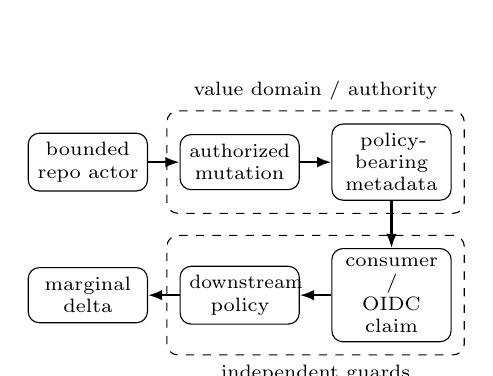
\begin{tikzpicture}[
  node distance=3.0mm and 4.0mm,
  box/.style={draw,rounded corners,align=center,font=\scriptsize,minimum height=7mm,text width=1.28cm},
  arr/.style={-{Latex[length=1.8mm]},thick}
]
\node[box] (a) {bounded\\repo actor};
\node[box,right=of a] (m) {authorized\\mutation};
\node[box,right=of m] (v) {policy-bearing\\metadata};
\node[box,below=6mm of v] (c) {consumer /\\OIDC claim};
\node[box,left=of c] (p) {downstream\\policy};
\node[box,left=of p] (d) {marginal\\delta};
\draw[arr] (a)--(m);
\draw[arr] (m)--(v);
\draw[arr] (v)--(c);
\draw[arr] (c)--(p);
\draw[arr] (p)--(d);
\node[draw,dashed,rounded corners,fit=(m)(v),inner sep=1.6mm,
      label={[font=\scriptsize]above:value domain / authority}] {};
\node[draw,dashed,rounded corners,fit=(c)(p),inner sep=1.6mm,
      label={[font=\scriptsize]below:independent guards}] {};
\end{tikzpicture}
\caption{Authority-provenance chain. A vulnerability exists only if an
actor-authorized mutation traverses a concrete deployed policy edge and creates
a new effective privilege or protection loss.}
\label{fig:chain}
\Description{A six-stage directed chain from a bounded repository actor through an authorized mutation, policy-bearing metadata, a consumer or OIDC claim, downstream policy, and a marginal security delta. Dashed boxes denote authority/value-domain constraints and independent guards.}
\end{figure}

\paragraph{Safe counterexamples.}
A mutable value can still be safe when (1) the actor lacks write authority, (2)
its domain has no protection-reducing value, (3) an independent guard remains
unsatisfied in every reachable state, (4) producer and consumer merely coexist,
or (5) the destination capability already exists initially.

\paragraph{Unknown.}
When the observation lacks editability, downstream policy, or deployment facts,
we return \N{} rather than inferring either safety or unsafety.  This design is
central to the public-repository evaluation, where organization schemas and
external trust policies are frequently private.

\paragraph{Witnesses and repair cuts.}
For \U{}, the analyzer returns a shortest mutation witness
$\pi=(m_1,\ldots,m_k)$.  A repair set $R$ is sufficient when it intersects every
unsafe witness path.  We compute both minimum-cardinality cuts and non-dominated
cuts under operator-supplied cost vectors.  This is a hitting-set formulation;
our contribution is the extraction of the cross-control-plane edges, not a new
hitting-set algorithm.

\section{Prototype}

Our prototype separates \emph{discovery} from
\emph{semantic decision}.  This separation became important during evaluation:
several early versions classified a known target correctly when supplied, yet
failed to find the target in a large repository.

\subsection{Evidence extraction}

Given an exact repository commit, the extractor looks for GitHub custom-property
definitions and values, workflow references through
\nolinkurl{github.event.repository.custom_properties}, organization-governance
configuration, ruleset targeting, OIDC property-claim configuration, and nearby
security consumers.  It records positive authority evidence (for example,
\nolinkurl{values_editable_by}), candidate consumer edges, protection-reducing
states, and independent guards.

The decision layer then applies the semantics in Section~\ref{sec:model}.  It
never upgrades an incomplete case to \U{} simply because a property has a
security-sounding name, nor to \Ssafe{} merely because a dangerous path was not
found.  Generated SDKs, API clients, fixtures, tests, examples, and vendored
libraries are tracked as provenance classes because they were a dominant source
of false positives at scale.

\subsection{Target-blind discovery}

For blind evaluation, the analyzer receives only case identifier, repository,
and exact commit.  Target property names and manual labels are withheld.  The
discovery pass ranks files and candidate properties using repository-tree and
content evidence, then invokes the same conservative semantic layer.  The
primary blind benchmark (V4) was frozen before a fresh 14-owner set was run, and
the target manifest was committed by SHA-256 before execution and revealed only
after the immutable raw artifact existed.

\subsection{Case aggregation}

A repository case is labeled \U{} if any candidate is \U{}, otherwise \Ssafe{}
if any candidate is \Ssafe{}, otherwise \N{}.  Infrastructure errors remain a
separate outcome and are never converted to \N{}.  This intentionally makes raw
positive errors visible in the scale study rather than hiding them under
abstention.

\section{Controlled Causal Experiments}
\label{sec:controlled}

We first establish that the modeled failure is not merely hypothetical.  Each
unsafe experiment holds repository code fixed and changes the minimum
policy-bearing state available to the bounded repository actor.  Table
\ref{tab:controlled} summarizes the paths.

\begin{table}[t]
\caption{Controlled experiments.  ``Delta'' is the observed change after only
the policy-bearing metadata is changed.}
\label{tab:controlled}
\small
\begin{tabularx}{\columnwidth}{@{}l l X@{}}
\toprule
ID & Class & Path and observed delta \\
\midrule
U1 & \U{} & \texttt{security\_tier}: GitHub OIDC $\rightarrow$ GCP WIF/IAM; project GET changes 403 $\rightarrow$ 200. \\
U2 & \U{} & Same property claim $\rightarrow$ JFrog dynamic mapping; repository GET changes 403 $\rightarrow$ 200. \\
U3 & \U{} & \texttt{security\_scan\_policy}: required check changes from blocked scan to successful bypass on the same revision. \\
U4 & \U{} & \texttt{branch\_protection\_profile}: repository exits an organization ruleset; an update previously denied becomes allowed. \\
S2 & \Ssafe{} & Repo-editable bypass selector plus org-only \texttt{security\_floor=enforced}; scan still blocks. \\
S3 & \Ssafe{} & Repo-editable \texttt{scan\_profile} limited to \{standard,hardened\}; both values preserve the gate. \\
\bottomrule
\end{tabularx}
\end{table}

\subsection{U1: GitHub property to Google Cloud}

We define a repository property \texttt{security\_tier} with values
\texttt{restricted} and \texttt{open}, permit the bounded repository actor to
change it, and include the property in GitHub's OIDC token.  A Google Cloud
Workload Identity Federation provider maps the resulting claim and an IAM
condition grants a harmless project-read capability only for the open value.
With the same workflow revision, the project GET is denied (HTTP 403) under
\texttt{restricted} and succeeds (HTTP 200) after the repository actor changes
only the property to \texttt{open}.  The actor cannot edit the GCP policy.

This experiment isolates the provenance problem: the downstream policy is
syntactically least-privilege, but the attribute used to select that privilege is
controlled by the workload's repository administrator.

\subsection{U2: the same producer reaches JFrog}

We repeat the producer side with the same textttt{security\_tier} property and
GitHub OIDC claim, but change the consumer to a JFrog OIDC dynamic-group mapping
and repository-read permission.  The target repository GET changes from 403 to
200 after only the property mutation.  Thus the issue is not specific to GCP
IAM semantics; the same upstream authority can propagate into an independent
artifact-service authorization plane.

\subsection{U3: required-check self-bypass}

U3 remains within GitHub.  A required security workflow reads
\texttt{security\_scan\_policy}.  Under \texttt{enforced}, a controlled unsafe
fixture causes the required check to fail.  The bounded actor changes only the
property to \texttt{bypass}; the same PR/commit then reports the required check
as successful without evaluating the fixture.  The branch rule has not changed,
but the actor controls the state that determines whether its required check
actually performs the intended protection.

\subsection{U4: property-selected organization ruleset}

GitHub organization rulesets can target repositories using custom-property
filters~\cite{github-rulesets}.  U4 defines a
\texttt{branch\_protection\_profile} with \texttt{protected} and
\texttt{excluded}.  The organization ruleset requires a pull request and
approval only for repositories matching \texttt{protected}.  With the property
repo-editable, changing it to \texttt{excluded} removes the repository from the
target set and enables an update previously denied.  This is policy-selection
self-authorization without an external cloud.

\subsection{Counterexperiments}

The safe controls show why ``mutable + consumed'' is not our rule.  S2 adds an
org-only \texttt{security\_floor=enforced}.  Even when the repository actor sets
the local selector to bypass, the fixture remains blocked.  S3 lets the actor
mutate a profile, but the allowed domain contains only \texttt{standard} and
\texttt{hardened}; neither disables the scan.  These controls directly motivate
$G$ and $D(x)$ in the formal model.

\section{Public Evidence and Blind Evaluation}

The controlled experiments establish causality but not whether the same
reasoning survives public repositories.  We therefore use three complementary
evaluations: a frozen semantic corpus, a target-blind benchmark, and a broad
noisy harvest.

\subsection{Frozen public semantic corpus}

We froze 12 public repository snapshots chosen to exercise concrete distinctions
in the model.  The corpus contains one strict \U{}, six \Ssafe{}, and five \N{}
cases.  The strict unsafe case is
\nolinkurl{mcp-research/mcp-security-scans}: a repository-editable
\texttt{GHAS\_Status\_Updated} property is used as scan state, and a recent
complete-looking value can suppress a rescan.  The safe cases include an
org-only property that selects a required-check lane, an org-only property that
selects organization rulesets, a mutable auto-merge opt-in whose independent
review/check protections remain, and a mutable property colocated with a
ruleset that actually targets a different criterion.

Five cases remain unknown because a decisive deployment fact is not public.  For
example, GoHarbor's \texttt{SKIP\_PROXY\_CACHE} visibly skips CI behavior, but
the frozen evidence does not establish who may edit the property.  We preserve
such cases as \N{} rather than guessing the organization schema.

On the original 11-case frozen corpus, the raw-evidence extractor reproduces all
11 strict labels; on the six binary cases this is 1 TP, 0 FP, 5 TN, and 0 FN.
This is a regression test on selected cases, not an accuracy estimate.  Simple
comparison rules demonstrate the semantic value of the additional conditions:
``repo-editable'' alone produces two false positives, while
``repo-editable + consumed'' still produces one.

\subsection{Blind V4: primary target-blind benchmark}
\label{sec:v4}

V4 is the primary auditable blind benchmark.  The analyzer was frozen, then 14
fresh repository snapshots from 14 previously unused owners were selected.  The
analyzer received only repository and exact commit.  A target-property manifest
was SHA-256 committed before the run and successfully verified after the raw
artifact was fixed.

The analyzer discovers the exact target in all 14 cases.  Strict manual labels
are 0 \U{} / 3 \Ssafe{} / 11 \N{}, while V4 predicts 0 / 2 / 12.  Semantic and
end-to-end agreement are therefore 13/14 (92.9\%), with zero false \U{} and zero
false \Ssafe{}.  The sole error is conservative: V413 is predicted \N{} even
though a captured organization-schema response explicitly records
\texttt{values\_editable\_by=org\_actors}, which is sufficient for \Ssafe{} under
our bounded actor model.

\begin{table}[t]
\caption{Complementary evaluation results.  None of the candidate-enriched sets
is an ecosystem prevalence sample.}
\label{tab:eval}
\small
\begin{tabularx}{\columnwidth}{@{}l r X@{}}
\toprule
Evaluation & Size & Main result \\
\midrule
Controlled & 6 & 4 causal \U{} paths; 2 live safe counterexperiments. \\
Public semantic corpus & 12 & 1 strict \U{}, 6 \Ssafe{}, 5 \N{}; selected regression corpus. \\
Blind V4 & 14 & target discovery 14/14; strict agreement 13/14 (92.9\%); 0 false \U{}/\Ssafe{}. \\
Blind V5 diagnostic & 14 & 12 scans complete; 11/12 semantic agreement; 1 conservative false \N{}, 2 transport errors. \\
Broad harvest & 699 & 698 scans complete; 1,993 raw candidates; 50-case frozen manual audit exposes positive-label noise. \\
\bottomrule
\end{tabularx}
\end{table}

\subsection{V5 diagnostic hardening}

The broad-scale analysis described next exposed a recurrent failure mode:
generated clients, tests, and reference schemas could look like affirmative safe
or unsafe deployment evidence.  We therefore froze a V5 deployment-provenance
gate and evaluated a fresh 14-owner candidate-enriched set.  Twelve cases
completed; two large repository reads failed with transport errors and remain
errors rather than being silently mapped to \N{}.

A historical cryptographic commitment to the original gold manifest exists, but
its exact manifest preimage was not durably retained.  We therefore do not claim
that the later reference labels open that commitment.  Instead, all 14 frozen
snapshots were independently re-adjudicated under the already-frozen U/S/N
rubric by an adjudicator blind to V5 predictions.  This superseding reference
set is 0 \U{} / 3 \Ssafe{} / 11 \N{}.  On the 12 completed cases V5 agrees on
11/12 (91.7\%), with no false \U{} or false \Ssafe{} and one conservative false
\N{}.  V5 correctly demotes a test/reference-style false-safe pattern, but misses
a fixed repository-identity guard in V501.  We therefore use V5 only as a
diagnostic validation; V4 remains the primary reveal-verifiable blind result.

\section{Broad Public-Code Realism Study}
\label{sec:scale}

Small blind sets cannot represent the noise of open-source code search.  We
therefore built two signature-driven candidate harvests whose canonical union
contains 699 repository+commit cases across 698 distinct repositories and 582
owners.  The set is intentionally candidate-enriched and is not random.  The
known strict public unsafe repository from the semantic corpus is absent from
the 699-case search universe, directly demonstrating that the harvest is not
exhaustive.

Frozen V4 completes on 698/699 cases and emits 1,993 candidate records: 9 raw
\U{}, 53 raw \Ssafe{}, and 1,931 raw \N{}.  Aggregated by repository case, this
becomes 4 \U{}, 15 \Ssafe{}, 679 \N{}, and one infrastructure error.  These raw
positives are triage signals, not vulnerability counts.

\subsection{Frozen 50-case manual audit}

Before manual labels were recorded, we froze a 50-case audit consisting of all
19 automatic-positive cases, one preselected real-automation boundary case, and
30 deterministic automatic-\N{} cases stratified by available protection and
consumer signals.  Manual strict labels are 0 \U{}, 3 \Ssafe{}, and 47 \N{}.
The resulting matrix is shown in Table~\ref{tab:matrix}.

\begin{table}[t]
\caption{Scale manual-audit confusion matrix.  Rows are strict manual labels and
columns are raw V4 case labels.  The selection deliberately includes every raw
positive case.}
\label{tab:matrix}
\centering
\small
\begin{tabular}{lrrrr}
\toprule
Manual $\backslash$ Auto & \U{} & \Ssafe{} & \N{} & Total \\
\midrule
\U{} & 0 & 0 & 0 & 0 \\
\Ssafe{} & 0 & 3 & 0 & 3 \\
\N{} & 4 & 12 & 31 & 47 \\
\midrule
Total & 4 & 15 & 31 & 50 \\
\bottomrule
\end{tabular}
\end{table}

Overall agreement is 34/50 (68\%), but this number must not be interpreted as
GitHub-wide accuracy because the sample intentionally overweights every raw
positive.  The more useful diagnostics are asymmetric.  All 31 selected raw-\N{}
cases remain manual \N{}, whereas all four raw \U{} cases are manual \N{} and
only 3/15 raw \Ssafe{} cases survive as strict \Ssafe{}.

\subsection{Why raw positives fail}

Manual audit identifies five recurring classes.

\begin{enumerate}[leftmargin=*,nosep]
  \item \textbf{Generated SDK/API material.}  The code accurately models
  GitHub custom-property APIs but does not establish that the repository deploys
  the modeled policy.
  \item \textbf{Tests and fixtures.}  Realistic property schemas and values
  appear in test data without a live protection consumer.
  \item \textbf{Provider/reference implementations.}  Terraform, Pulumi,
  Crossplane, and language clients expose authority-relevant fields but do not
  instantiate the downstream composition.
  \item \textbf{Unrelated custom properties.}  Simulation, robotics, graph, or
  application metadata matches generic vocabulary while having nothing to do
  with GitHub repository policy.
  \item \textbf{Generic security vocabulary.}  Security-like names can occur in
  documentation or configuration without a real producer-to-consumer edge.
\end{enumerate}

The three manual-safe cases illustrate the opposite: MIT Open Learning uses an
org-only \texttt{tier} property to select organization rulesets;
OpenTelemetry consumes repository properties as telemetry metadata; and Team
Immersive Intelligence uses a property as a Discord/display name.  These are
relevant deployed uses, but affirmative evidence blocks any new bounded-actor
privilege.

The preselected boundary case
\nolinkurl{github/actions-migrations-via-copilot} is also instructive.  A
repo-editable \texttt{GH\_MIGRATION\_TYPE} value selects real migration/Copilot
automation, so both mutation authority and a deployed downstream effect are
present.  It remains \N{} because the frozen evidence does not establish a new
security privilege or protection loss.  Treating every metadata-controlled
automation as security-sensitive would therefore overclassify real systems.

\subsection{Strict public U and contextual U*}

Across the focused public review, we retain one strict public \U{} and four
contextual \emph{U*} cases.  U* is narrative-only and remains \N{} in all
benchmark metrics: it denotes a public, concrete security effect for which
exactly one decisive deployment fact, typically editability or a private
external policy, is unavailable.  Examples include StepSecurity's
custom-property opt-out for Harden-Runner and GoHarbor's property-controlled CI
skip.  This notation lets us discuss plausible real deployment risk without
turning missing private organization state into fabricated ground truth.

\section{Repair Synthesis}

Detection is more useful when it identifies where to break the path.  For each
controlled unsafe composition we encode candidate cuts and relative operator
costs.  Example cuts include making \texttt{security\_tier} org-only, adding an
independently controlled GCP or JFrog condition, adding the S2 org-only security
floor, restricting the U3 selector to a safe value domain as in S3, making the
U4 profile org-only, or retaining a baseline ruleset whose applicability does
not depend on the mutable selector.

For a set of unsafe witness paths $\mathcal{P}$, a repair $R$ is sufficient when
$R$ intersects every $\pi\in\mathcal{P}$.  Our transparent prototype enumerates
feasible subsets and returns both minimum-cardinality sets and a Pareto frontier
over supplied cost dimensions such as automation disruption, administrative
scope, repositories affected, and downstream systems changed.  We deliberately
do not assign dollar costs or claim the supplied relative vectors are measured
operational costs.

The controlled bundle provides two live post-condition demonstrations: S2
empirically validates the fixed-floor repair for U3, and S3 validates the
safe-domain repair.  The public MIT \texttt{tier} case independently supports
the org-only boundary used as one U4 repair.  External GCP/JFrog policy changes
and organization-admin property mutations are represented as executable repair
models but are not claimed as live post-repair reruns.

A useful consequence is that the smallest repair need not be the most desirable.
Centralizing one upstream property can cut multiple downstream paths in one
change, while two narrower downstream guards may preserve legitimate repository
automation with lower disruption.  Reporting a Pareto frontier exposes this
tradeoff instead of prescribing ``make everything org-only.''

\section{Discussion}

\subsection{What the results establish}

The controlled experiments answer RQ1 affirmatively: policy-bearing repository
metadata can create real cross-control-plane privilege and protection deltas,
including two external authorization systems and two GitHub-native protections.
The counterexperiments show that editability and consumption are insufficient
conditions.

For RQ2, blind V4 demonstrates that a frozen target-blind analyzer can recover
the intended property in a small fresh-owner set while remaining conservative:
its only semantic miss is an abstention where org-only authority was present in
a captured schema.  V5 provides a separate diagnostic showing that
deployment-provenance filtering removes an observed reference/test failure mode
but does not eliminate all conservative misses.

RQ3 produces the most cautionary result.  Broad search creates many structurally
plausible positives that are not deployed compositions.  A tool that reports
raw SDK/test/reference matches as vulnerabilities would have poor positive
precision in our deliberately positive-enriched manual audit.  Conversely, the
selected raw-\N{} cases are strongly conservative.  This asymmetry suggests a
practical architecture: broad static search for triage, followed by
provenance-aware evidence joining before a positive security claim.

For RQ4, path-cut repair synthesis provides concrete alternatives whose semantics
are tied to the unsafe witness.  The repair engine itself is simple; its value is
that upstream authority boundaries and downstream independent guards become
comparable cuts in the same composed path.

\subsection{Why this is not just ABAC or an attack graph}

GitHub's property features are naturally attribute-based, and our reachability
model resembles established attack-graph formulations.  We do not claim a new
general ABAC or graph theory.  The empirical and systems contribution is the
join across \emph{who may mutate an attribute}, \emph{how that attribute is
materialized or propagated by CI/CD}, \emph{which independently administered
policy consumes it}, and \emph{whether the composed result creates a marginal
security delta}.  Existing authorization-provenance work asks how an
authorization was derived~\cite{hu2010authprov}; our focus is whether an actor
can alter the provenance inputs that cause a different authorization to be
derived across operational control planes.

Likewise, software-supply-chain provenance systems such as in-toto and SLSA
record how artifacts were produced and support integrity verification
~\cite{torresarias2019intoto,slsa12}.  Our use of provenance is complementary:
we track the authority provenance of policy-bearing state that governs the build
or deployment rather than the production history of the resulting artifact.

\subsection{Operational implications}

The obvious blanket defense---make every security-relevant property org-only---
is safe but can defeat the delegation that custom properties were introduced to
support.  A less disruptive rule is: \emph{a principal should not control every
input needed to select a stronger authority state for itself}.  This can be
implemented upstream (org-only property), downstream (independent immutable
condition), through domain design (no reducing value), or through a fixed
baseline protection that does not depend on the mutable selector.

Cloud OIDC deserves particular attention because it turns repository metadata
into signed identity claims.  Cryptographic authenticity answers ``did GitHub
issue this claim?''; it does not answer ``was the claim value controlled by a
principal that the relying policy intended to constrain?''  The latter is an
authorization-provenance question.

\section{Limitations and Ethics}

\paragraph{GitHub-only evaluation.}
We study GitHub because its custom properties, Actions OIDC, and organization
rulesets provide several independent consumers of the same metadata abstraction.
The formal model is platform-agnostic, but we do not claim empirical
cross-platform generality.  GitLab, Azure DevOps, and other CI/CD platforms are
future validation targets.

\paragraph{Public observability.}
Organization schemas, rulesets, and external IAM policies are often private.
Strict \U{} therefore requires stronger public evidence than a real attacker
inside an organization would need.  Our \N{} and U* categories are designed to
make this limitation visible rather than fill gaps with assumptions.

\paragraph{Sampling.}
Neither the 14-case blind sets nor the 699-case harvest are random samples of
GitHub.  The harvest is signature-driven and demonstrably misses the known
strict public \U{}.  We make no prevalence claim.

\paragraph{Ground truth and V5.}
V4's target manifest is cryptographically committed and successfully revealed.
For V5, the historical commitment remains but the exact original preimage was
lost.  The later reference labels were independently adjudicated blind to V5
predictions and are explicitly treated as a superseding diagnostic reference,
not as a recovered precommitment.  This distinction does not affect the primary
V4 result.

\paragraph{Controlled impact.}
Unsafe experiments use repositories and cloud/artifact resources controlled by
the researchers, harmless read capabilities or controlled fixtures, and
bounded accounts.  We do not modify third-party repositories or attempt to
exercise suspected public paths against private organization state.

\section{Related Work}

\paragraph{Closest public tooling.}
We also inspected three public tools that overlap materially with individual
parts of our pipeline.  \nolinkurl{gha-oidc-auditor} understands GitHub OIDC trust
and explicitly synthesizes custom-property OIDC claims, but in the inspected
snapshot we found no handling of the upstream
\nolinkurl{values_editable_by} authority boundary~\cite{gha-oidc-auditor}.
\nolinkurl{tap-plugin-github-core} collects custom-property allowed values and
editability and models GitHub federation edges, while its documentation states
that downstream cloud trust conditions and permissions are outside the
observable GitHub-side graph~\cite{tap-github-core}.  \nolinkurl{github-config}
provides strong declarative GitHub governance and flags widening property
editability as protection weakening, but explicitly leaves external/cloud
controls outside its owned boundary~\cite{mindclade-config}.  These systems
already cover important pieces, so our novelty claim is deliberately narrower:
joining mutation authority to a deployed consumer, downstream authorization or
protection semantics, and a \emph{marginal} effective delta, while retaining
unknowns, witnesses, and repair cuts.

\paragraph{GitHub Actions and CI/CD security.}
Koishybayev et al. analyze 447,238 GitHub workflows and identify widespread
workflow overprivilege, unsafe triggers, and third-party Action risk
~\cite{koishybayev2022gha}.  More recent studies measure security-practice
adoption, workflow evolution, documentation quality, and self-hosted-runner
risk~\cite{kubo2026action,boschanski2026docs,shi2026shcrguard,rostami2026evolution}.
These works motivate the importance of CI/CD as a security boundary.  Our focus
is different: we hold workflow code fixed and analyze authority that propagates
through policy-bearing metadata into GitHub-native or external authorization
systems.

\paragraph{Attribute-based access control and policy composition.}
ABAC explicitly makes authorization depend on subject, object, action, and
environment attributes~\cite{hu2015abac}.  Prior work studies authorization
provenance and policy composition in distributed settings
~\cite{hu2010authprov,lin2009abaccomposition}.  We build on these ideas but treat
attribute \emph{mutation authority} as a first-class edge and evaluate its
practical composition across repository, CI/CD, OIDC, cloud, and artifact
control planes.

\paragraph{Attack graphs and remediation.}
Attack graphs represent multi-step causal paths and support security hardening;
recent surveys summarize a large literature on automated generation
~\cite{konsta2024attackgraphs}.  We similarly use reachability and path cuts, but
our graph is deliberately narrow: it is extracted from policy-bearing metadata
and its consumers, and a path is considered unsafe only when it changes the
marginal effective privilege/protection state of the bounded actor or workload.

\paragraph{Supply-chain provenance.}
in-toto and SLSA provide provenance and integrity guarantees for software
artifacts and build processes~\cite{torresarias2019intoto,slsa12}.  Our
``authority provenance'' asks a different question: which principal controls
the metadata that later governs authorization.  Artifact provenance can be
cryptographically sound while the policy that decides who may produce or deploy
an artifact still trusts a self-controlled attribute.

\section{Conclusion}

Repository metadata is increasingly part of the authorization surface.  When a
bounded repository actor can change a value that later selects a ruleset,
changes a required security gate, or becomes an OIDC attribute trusted by an
external service, local least-privilege configurations can compose into
self-authorization.  We show four such paths causally, formalize the required
mutation-to-delta chain, and demonstrate why safe domains, independent guards,
and honest unknowns are necessary to avoid simplistic findings.

The evaluation also exposes an important negative result: broad public-code
search produces many convincing but non-deployed positives.  Generated SDKs,
tests, providers, and security-like vocabulary cannot substitute for deployment
provenance.  A practical analyzer should therefore be conservative, produce
short evidence-backed witnesses, and make uncertainty explicit.  Finally,
repair cuts show that the same compositional model can support remediation by
breaking authority upstream, adding an independent condition downstream, or
constraining the reachable value domain.

\bibliographystyle{ACM-Reference-Format}
\begin{thebibliography}{18}

\bibitem{koishybayev2022gha}
Igibek Koishybayev, Aleksandr Nahapetyan, Raima Zachariah, Siddharth Muralee,
Bradley Reaves, Alexandros Kapravelos, and Aravind Machiry. 2022.
Characterizing the Security of GitHub CI Workflows. In \emph{31st USENIX
Security Symposium (USENIX Security 22)}, 2747--2764.

\bibitem{kubo2026action}
Yusuke Kubo, Fumihiro Kanei, Mitsuaki Akiyama, Takuro Wakai, and Tatsuya Mori.
2026. Action Required: A Mixed-Methods Study of Security Practices in GitHub
Actions. In \emph{Network and Distributed System Security Symposium (NDSS)}.

\bibitem{boschanski2026docs}
Lukas Boschanski and Marco Vieira. 2026. Evaluating CI/CD Security Best
Practices in the GitHub Actions Documentation. In \emph{20th International
Symposium on Empirical Software Engineering and Measurement (ESEM)}.
DOI: 10.4230/LIPIcs.ESEM.2026.15.

\bibitem{shi2026shcrguard}
Pengfei Shi, Jiaqi Huang, Yifan Xu, Jinfu Chen, Jie Lu, Fangyuan Qi, and Hanzhong
Peng. 2026. SHCRGuard: Security Risk Analysis of Self-hosted CI/CD Runners in
GitHub Actions. \emph{Journal of Systems and Software} 241 (2026), 113018.
DOI: 10.1016/j.jss.2026.113018.

\bibitem{rostami2026evolution}
Pooya Rostami Mazrae, Alexandre Decan, Tom Mens, and Mairieli Wessel. 2026. An
Empirical Study of the Evolution of GitHub Actions Workflows. \emph{Journal of
Systems and Software} 236 (2026), 112824. DOI: 10.1016/j.jss.2026.112824.

\bibitem{hu2010authprov}
Jinwei Hu, Yan Zhang, Ruixuan Li, and Zhengding Lu. 2010. A Logic for
Authorization Provenance. In \emph{Proceedings of the 5th ACM Symposium on
Information, Computer and Communications Security (ASIACCS)}, 238--249.
DOI: 10.1145/1755688.1755718.

\bibitem{hu2015abac}
Chung Tong Hu, David F. Ferraiolo, David R. Kuhn, Raghu N. Kacker, and Yu Lei.
2015. Implementing and Managing Policy Rules in Attribute Based Access Control.
In \emph{2015 IEEE 16th International Conference on Information Reuse and
Integration (IRI)}, 518--525. DOI: 10.1109/IRI.2015.98.

\bibitem{lin2009abaccomposition}
L. Lin, J. Huai, and X. Li. 2009. Attribute-Based Access Control Policies
Composition Algebra. \emph{Journal of Software} 20, 2 (2009), 403--414.
DOI: 10.3724/SP.J.1001.2009.00403.

\bibitem{konsta2024attackgraphs}
Alyzia-Maria Konsta, Alberto Lluch Lafuente, Beatrice Spiga, and Nicola Dragoni.
2024. Survey: Automatic Generation of Attack Trees and Attack Graphs.
\emph{Computers \& Security} 137 (2024), 103602.
DOI: 10.1016/j.cose.2023.103602.

\bibitem{torresarias2019intoto}
Santiago Torres-Arias, Hammad Afzali, Trishank Karthik Kuppusamy, Reza Curtmola,
and Justin Cappos. 2019. in-toto: Providing Farm-to-Table Guarantees for Bits
and Bytes. In \emph{28th USENIX Security Symposium (USENIX Security 19)}, 1393--1410.

\bibitem{slsa12}
SLSA Community. 2026. Supply-chain Levels for Software Artifacts (SLSA)
Specification, Version 1.2. \url{https://slsa.dev/spec/v1.2/}.

\bibitem{github-custom-properties}
GitHub. 2026. Managing Custom Properties for Repositories in Your Organization.
\url{https://docs.github.com/en/organizations/managing-organization-settings/managing-custom-properties-for-repositories-in-your-organization}.

\bibitem{github-custom-properties-api}
GitHub. 2026. REST API Endpoints for Custom Properties.
\url{https://docs.github.com/en/rest/orgs/custom-properties}.

\bibitem{github-rulesets}
GitHub. 2026. Creating Rulesets for Repositories in Your Organization.
\url{https://docs.github.com/en/organizations/managing-organization-settings/creating-rulesets-for-repositories-in-your-organization}.

\bibitem{github-oidc-properties}
GitHub. 2026. OpenID Connect: Using Repository Custom Properties as OIDC Claims.
\url{https://docs.github.com/en/actions/concepts/security/openid-connect}.

\bibitem{gha-oidc-auditor}
gamesapeca. 2026. \nolinkurl{gha-oidc-auditor}, snapshot
\nolinkurl{d86257b70d84}.
\url{https://github.com/gamesapeca/gha-oidc-auditor}.

\bibitem{tap-github-core}
unified-systems-com. 2026. \nolinkurl{tap-plugin-github-core}, snapshot
\nolinkurl{a163c29c028c}.
\url{https://github.com/unified-systems-com/tap-plugin-github-core}.

\bibitem{mindclade-config}
mindclade. 2026. \nolinkurl{github-config}, snapshot
\nolinkurl{d2071e9e477b}.
\url{https://github.com/mindclade/github-config}.

\end{thebibliography}

\clearpage
\appendix
\section{Evaluation Provenance Summary}

Table~\ref{tab:prov} records the evaluation boundaries that are easy to blur in
a short paper.  V4 is the primary blind benchmark because both the frozen
analyzer and precommitted target manifest are reveal-verifiable.  V5 is retained
because it directly tests the deployment-provenance failure class discovered by
the broad audit, but its superseding blind adjudication is not represented as
the recovered historical gold preimage.

\begin{table}[h]
\caption{Evaluation provenance and reporting boundary.}
\label{tab:prov}
\small
\begin{tabularx}{\columnwidth}{@{}l X@{}}
\toprule
Component & Reporting boundary \\
\midrule
Controlled U/S & Causal demonstrations in researcher-controlled resources; not prevalence. \\
Public semantic corpus & Selected regression cases; exact frozen commits; not discovery accuracy. \\
Blind V4 & Frozen analyzer; fresh owners; target manifest cryptographically committed and later verified. \\
Blind V5 & Frozen analyzer; fresh owners; independent prediction-blind superseding adjudication; historical preimage unrecovered. \\
699 harvest & Signature-driven realism universe; not exhaustive or random. \\
50-case audit & Frozen positive-enriched manual sample; agreement is not ecosystem accuracy. \\
\bottomrule
\end{tabularx}
\end{table}

\section{Strict Decision Checklist}

For each candidate, the manual and automated reasoning use the following order:
(1) identify the exact policy-bearing property/configuration; (2) determine
whether the bounded repository actor can mutate it; (3) establish a concrete
deployed consumer; (4) determine reachable security-reducing values; (5) check
independent guards; (6) compare the resulting effective privilege/protection
state with the baseline; and (7) retain \N{} when any decisive deployment fact
is missing.  Generated, test, documentation, provider, vendor, and unrelated
metadata are never promoted to deployed \U{} without separate evidence.

\end{document}
